%
% main.tex -- Paper zum Thema verzoegerte Differentialgleichung
%
% (c) 2018 Raphael Unterer, Hochschule Rapperswil
%
\chapter{Numerische Lösung einer verzögerten Differentialgleichung\label{chapter:verzoegert}}
\lhead{Numerische Lösung einer verzögerten Differentialgleichung}
\begin{refsection}
\chapterauthor{Raphael Unterer}

\section{Einleitung}
Verzögerte Differentialgleichungen sind gewöhnliche Differentialgleichungen, bei welchen die Ableitung von früheren Funktionswerten abhängt.
Ein gutes Beispiel dafür ist die Populationsentwicklung in der Biologie. 
Für das Populationswachstum bei Tieren ist entscheidend wie viele junge Tiere geschlechtsreif werden.
Somit hängt das Wachstum von einem früheren Wachstum ab, da es einige Zeit dauert bis die Jungen geschlechtsreif sind.
Es gibt diverse weitere Anwendungen für verzögerte Differentialgleichungen in Physik, Chemie und Biologie (vgl. \cite{verzoegert:erneux}).

Hier wollen wir vor allem die verzögerte Differentialgleichung zur Modellierung des El Niño Phänomens \eqref{elninodde:2} betrachten.
Wir lernen zuerst einige grundlegende Methoden kennen, um eine verzögerte Differentialgleichung analytisch zu untersuchen. 
Danach wird gezeigt, wie eine numerische Berechnung gemacht wird.

%
% main.tex -- Paper zum Thema verzoegerte Differentialgleichung
%
% (c) 2018 Raphael Unterer, Hochschule Rapperswil
%
\section{Grundlagen verzögerte Differentialgleichungen}
\rhead{Grundlagen DDE}
\subsection{Definitionen}


\begin{definition}
	Eine allgemeine verzögerte Differentialgleichung 1. Ordnung sieht folgendermaßen aus:
	\begin{equation}
		\dot{x}(t) = f(x(t),x(t-\tau_1),\dots,x(t-\tau_n)).
	\end{equation}
	Dabei ist $f$ eine beliebige Funktion. Die Verzögerungen $\tau_1,\dots,\tau_n$ sind gegeben und nach der Grösse geordnet, also $0<\tau_1<\dots<\tau_n$.
\end{definition}
Verzögerte Differentialgleichungen werden als DDE (engl. "\textbf{D}elayed \textbf{D}ifferential \textbf{E}quation") abgekürzt.

Im Unterschied zu einer gewöhnlichen Differentialgleichung ist das Anfangswertproblem nicht mehr eindimensional, d.h. es genügt nicht mehr den Anfangszustand zu kennen.
Alle Werte von $-\tau_n$ bis $0$ müssen gegeben sein. 
Es braucht nicht nur einen einzelnen Anfangswertvektor, sondern eine ganze Funktion von Anfangswertvektoren im Intervall $[-\tau_n, 0]$.

\subsection{Analytische Lösungsverfahren an einem Beispiel}
Um die analytischen Lösungsverfahren zu verstehen, werden diese zunächst an einem einfachen Beispiel erläutert.
In den folgenden Betrachtungen analysieren wir die DDE:
\begin{equation}\label{bsp}
\dot{y}(t)=ky(t-\tau).
\end{equation}

\subsubsection{Schrittweises Lösen}
Beim schrittweisen Lösen wird die DDE immer in Schritten von einem $\tau$ gelöst.
Wir nehmen an, dass $y$ im Bereich von $-\tau$ bis $0$ immer konstant bleibt.
Somit haben wir die folgende Funktion der Anfangswerte:
\begin{equation}
	y(t)=1 \quad\text{wenn}\quad -1\le t<0.
\end{equation}
Daraus folgt, dass im Bereich von $0\le t<\tau$ die Ableitung
\begin{equation}\label{abl}
	\dot{y}(t)=k
\end{equation}
wird. Durch Integrieren von \eqref{abl} erhalten wir
\begin{equation}\label{schritt1}
	y(t)=1+kt
\end{equation}
für den Bereich $0\le t<\tau$. 
Dieses $y(t)$ kann als Anfangswert für den nächsten Schritt genommen werden.
Wir erhalten für den zweiten Schritt  $\tau\le t<2\tau$ 
\begin{equation}\label{abl2}
	\dot{y}(t)=k(1+k(t-\tau))=k+k^2(t-\tau).
\end{equation}
Es ist offensichtlich, dass diese Methode nur für kurze Zeiten, einfache Anfangswerte und einfache Formeln funktioniert. 
Bereits \eqref{abl2} ist nicht mehr ganz einfach zu integrieren. 
Für längere Zeiten werden die Integrale immer komplexer.

In Abbildung \ref{fig:bsp} sieht man die Lösung für das Beispiel \eqref{bsp}. 
Die lineare Funktion \eqref{schritt1} ist als erster Schritt gut sichtbar.
Ab Schritt 2 ist die Lösung nicht mehr eine lineare Funktion, sondern eine Polynomfunktion höheren Grades. 
\begin{figure}
	\centering
	% This file was created by matlab2tikz.
%
%The latest updates can be retrieved from
%  http://www.mathworks.com/matlabcentral/fileexchange/22022-matlab2tikz-matlab2tikz
%where you can also make suggestions and rate matlab2tikz.
%
\begin{tikzpicture}

\begin{axis}[%
width=4.521in,
height=3.566in,
at={(0.758in,0.481in)},
scale only axis,
xmin=-1,
xmax=3,
ymin=-1,
ymax=2,
ylabel={$y$},
xlabel={$t$},
axis background/.style={fill=white}
]
\addplot [color=blue, forget plot]
  table[row sep=crcr]{%
0	1\\
0.03000300030003	0.970000000000003\\
0.06000600060006	0.940000000000007\\
0.09000900090009	0.91000000000001\\
0.12001200120012	0.880000000000013\\
0.15001500150015	0.850000000000017\\
0.18001800180018	0.82000000000002\\
0.21002100210021	0.790000000000023\\
0.24002400240024	0.760000000000026\\
0.27002700270027	0.73000000000003\\
0.3000300030003	0.700000000000033\\
0.33003300330033	0.670000000000036\\
0.36003600360036	0.64000000000004\\
0.39003900390039	0.610000000000043\\
0.42004200420042	0.580000000000046\\
0.45004500450045	0.55000000000005\\
0.48004800480048	0.520000000000053\\
0.51005100510051	0.490000000000054\\
0.54005400540054	0.460000000000052\\
0.57005700570057	0.43000000000005\\
0.6000600060006	0.400000000000048\\
0.63006300630063	0.370000000000045\\
0.66006600660066	0.340000000000043\\
0.69006900690069	0.310000000000041\\
0.72007200720072	0.280000000000039\\
0.75007500750075	0.250000000000036\\
0.78007800780078	0.220000000000037\\
0.81008100810081	0.190000000000037\\
0.84008400840084	0.160000000000038\\
0.87008700870087	0.130000000000038\\
0.9000900090009	0.100000000000039\\
0.93009300930093	0.0700000000000395\\
0.96009600960096	0.0400000000000395\\
0.99009900990099	0.0100000000000394\\
1.02010201020102	-0.0198069499999607\\
1.05010501050105	-0.0487674499999608\\
1.08010801080108	-0.076827949999961\\
1.11011101110111	-0.103988449999961\\
1.14011401140114	-0.130248949999962\\
1.17011701170117	-0.155609449999962\\
1.2001200120012	-0.180069949999963\\
1.23012301230123	-0.203630449999964\\
1.26012601260126	-0.226290949999964\\
1.29012901290129	-0.248051449999965\\
1.32013201320132	-0.268911949999966\\
1.35013501350135	-0.288872449999967\\
1.38013801380138	-0.307932949999969\\
1.41014101410141	-0.32609344999997\\
1.44014401440144	-0.343353949999971\\
1.47014701470147	-0.359714449999973\\
1.5001500150015	-0.375174949999974\\
1.53015301530153	-0.389735449999976\\
1.56015601560156	-0.403395949999978\\
1.59015901590159	-0.416156449999979\\
1.62016201620162	-0.42801694999998\\
1.65016501650165	-0.438977449999982\\
1.68016801680168	-0.449037949999983\\
1.71017101710171	-0.458198449999984\\
1.74017401740174	-0.466458949999985\\
1.77017701770177	-0.473819449999987\\
1.8001800180018	-0.480279949999988\\
1.83018301830183	-0.485840449999989\\
1.86018601860186	-0.49050094999999\\
1.89018901890189	-0.494261449999991\\
1.92019201920192	-0.497121949999992\\
1.95019501950195	-0.499082449999993\\
1.98019801980198	-0.500142949999995\\
2.01020102010201	-0.500303583919996\\
2.04020402040204	-0.499574065819996\\
2.07020702070207	-0.497979917719998\\
2.1002100210021	-0.495548139619999\\
2.13021302130213	-0.49230573152\\
2.16021602160216	-0.488279693420001\\
2.19021902190219	-0.483497025320003\\
2.22022202220222	-0.477984727220004\\
2.25022502250225	-0.471769799120005\\
2.28022802280228	-0.464879241020006\\
2.31023102310231	-0.457340052920007\\
2.34023402340234	-0.449179234820008\\
2.37023702370237	-0.440423786720009\\
2.4002400240024	-0.43110070862001\\
2.43024302430243	-0.421237000520011\\
2.46024602460246	-0.410859662420012\\
2.49024902490249	-0.399995694320012\\
2.52025202520252	-0.388672096220013\\
2.55025502550255	-0.376915868120014\\
2.58025802580258	-0.364754010020014\\
2.61026102610261	-0.352213521920015\\
2.64026402640264	-0.339321403820016\\
2.67026702670267	-0.326104655720016\\
2.7002700270027	-0.312590277620017\\
2.73027302730273	-0.298805269520017\\
2.76027602760276	-0.284776631420018\\
2.79027902790279	-0.270531363320018\\
2.82028202820282	-0.256096465220018\\
2.85028502850285	-0.241498937120018\\
2.88028802880288	-0.226765779020019\\
2.91029102910291	-0.211923990920019\\
2.94029402940294	-0.197000572820019\\
2.97029702970297	-0.182022524720019\\
};
\addplot [color=blue, forget plot]
  table[row sep=crcr]{%
-1	1\\
0	1\\
};
\addplot [dashed,color=black, forget plot]
table[row sep=crcr]{%
	0	-1\\
	0	2\\
};
\addplot [dashed,color=black, forget plot]
table[row sep=crcr]{%
	1	-1\\
	1	2\\
};
\addplot [dashed,color=black, forget plot]
table[row sep=crcr]{%
	2	-1\\
	2	2\\
};
\end{axis}
\end{tikzpicture}%
	\caption{Beispiel mit $k=-1$ und $\tau=1$}
	\label{fig:bsp}
\end{figure}

\subsubsection{Charakteristische Gleichung}
Bei gewöhnlichen Differentialgleichungen können Lösungen mit Hilfe des charakteristischen Polynoms gefunden werden. 
Bei DDEs wird das Polynom zu einer Gleichung. 
Wir betrachten wiederum die Gleichung \eqref{bsp} und verwenden als Lösungsansatz
\begin{equation}\label{ansatz}
	y(t) = ce^{\lambda t}.
\end{equation}
Dieser klassische Ansatz eignet sich (fast) immer, da die Exponentialfunktion beim Differenzieren erhalten bleibt. 
\eqref{ansatz} eingesetzt in \eqref{bsp} ergibt
\begin{equation}
	\lambda ce^{\lambda t} = kce^{\lambda (t-\tau )}.
\end{equation} 
Diese Gleichung kann durch $ce^{\lambda t}$ gekürzt werden zu
\begin{equation}\label{chareq}
	\lambda  - ke^{-\lambda \tau}= 0.
\end{equation} 
Damit können nun verschiedene Werte für die Konstante $k$ berechnet werden, je nachdem wie die Lösung $\lambda$ aussehen soll.
Wir nehmen an, dass $\lambda$ komplex ist und setzen $\lambda = \lambda_r + i\lambda_i$ in die Gleichung \eqref{chareq} ein.
\begin{equation}\label{chareq_kompl}
	\lambda_r + i\lambda_i  - ke^{-(\lambda_r + i\lambda_i) \tau}= 0
\end{equation} 
Real- und Imaginärteil dieser Gleichung können wir mit Hilfe der eulerschen Formel $e^{iy}=\cos(y)+i\sin(y)$ trennen und erhalten
\begin{align}
	\lambda_r - ke^{-\lambda_r\tau}\cos(\lambda_i\tau)&=0 \label{realchar} \\
	\lambda_i + ke^{-\lambda_r\tau}\sin(\lambda_i\tau)&=0 \label{imagchar}.
\end{align}
Nimmt man den zweiten Term auf die rechte Seite und dividiert die beiden Gleichungen, erhält man
\begin{equation} \label{chareq_kompl_frac}
	-\frac{\lambda_r}{\lambda_i} = \cot(\lambda_i\tau).
\end{equation}
Damit lassen sich nun beliebig viele Kombinationen von $\lambda$ und $k$ generieren.
Als Beispiel wollen wir eine periodische Schwingung mit gleichbleibender Amplitude erreichen.
Daraus ergibt sich ein $\lambda_r = 0$. 
Die Verzögerung ist gegeben als $\tau = 1$.
Eingesetzt in \eqref{chareq_kompl_frac} erhalten wir:
\begin{equation}
	\cot(\lambda_i) = 0 \qquad\Rightarrow\qquad \lambda_i = (2n-1)\frac{\pi}{2}.
\end{equation}
Mit $n\in \mathbb{N}$ können wir z.B. die kleinste Frequenz $n=1$ einsetzen und erhalten $\lambda_i = \frac{\pi}{2}$.
Damit können wir aus \eqref{imagchar} die Konstante $k$ bestimmen.
\begin{equation}
	\frac{\pi}{2} + k = 0 \qquad\Rightarrow\qquad k = -\frac{\pi}{2}
\end{equation}
Zur Überprüfung wurde mit diesen Werten die Gleichung numerisch berechnet (vgl. Abbildung \ref{fig:bsp_chareq}).
Man sieht dort gut die gleichbleibende Amplitude und die Periodendauer von $\frac{2\pi}{\frac{\pi}{2}}=4$.

\begin{figure}
	\centering
	% This file was created by matlab2tikz.
%
%The latest updates can be retrieved from
%  http://www.mathworks.com/matlabcentral/fileexchange/22022-matlab2tikz-matlab2tikz
%where you can also make suggestions and rate matlab2tikz.
%
\begin{tikzpicture}

\begin{axis}[%
width=4.521in,
height=3.566in,
at={(0.758in,0.481in)},
scale only axis,
xmin=-1,
xmax=20,
ymin=-2,
ymax=2,
ylabel={$y$},
xlabel={$t$},
axis background/.style={fill=white}
]
\addplot [color=blue, forget plot]
  table[row sep=crcr]{%
0	1\\
0.2000200020002	0.685840734641018\\
0.4000400040004	0.371681469282036\\
0.6000600060006	0.0575222039230558\\
0.8000800080008	-0.256637061435924\\
1.000100010001	-0.570796326794905\\
1.2001200120012	-0.8370781412042\\
1.4001400140014	-1.004673781207\\
1.6001600160016	-1.07357337719891\\
1.8001800180018	-1.04377692917992\\
2.000200020002	-0.91528443715004\\
2.2002200220022	-0.692811831767233\\
2.4002400240024	-0.401719394778529\\
2.6002600260026	-0.0730132788391235\\
2.8002800280028	0.262300239370685\\
3.000300030003	0.573214883170596\\
3.2003200320032	0.829061882795288\\
3.4003400340034	1.00375096899054\\
3.6003600360036	1.08044888928263\\
3.8003800380038	1.05206329884011\\
4.000400040004	0.921242761934929\\
4.2004200420042	0.700358046775638\\
4.4004400440044	0.410894972395743\\
4.6004600460046	0.0811695702016152\\
4.8004800480048	-0.256698001198943\\
5.000500050005	-0.56984365282742\\
5.2005200520052	-0.827718726631608\\
5.4005400540054	-1.00508644212531\\
5.6005600560056	-1.08457724034126\\
5.8005800580058	-1.05837694192613\\
6.000600060006	-0.928955575193748\\
6.2006200620062	-0.708834845900301\\
6.4006400640064	-0.419399587351868\\
6.6006600660066	-0.0888208309815821\\
6.8006800680068	0.250697886833838\\
7.000700070007	0.566058621725787\\
7.2007200720072	0.826489603116091\\
7.4007400740074	1.0065466558522\\
7.6007600760076	1.08860232292087\\
7.8007800780078	1.06457222915751\\
8.000800080008	0.936709891836633\\
8.2008200820082	0.717395204334429\\
8.4008400840084	0.427936675271025\\
8.6008600860086	0.0965014634190242\\
8.8008800880088	-0.244625951676723\\
9.000900090009	-0.562188709016319\\
9.2009200920092	-0.825199586034987\\
9.4009400940094	-1.007964533518\\
9.6009600960096	-1.09259284835939\\
9.8009800980098	-1.0707485030828\\
10.00100010001	-0.944471114793201\\
10.2010201020102	-0.725985834900832\\
10.4010401040104	-0.436519896039718\\
10.6010601060106	-0.104240311052822\\
10.8010801080108	0.238486952445908\\
11.001100110011	0.558249593995494\\
11.2011201120112	0.823846299489424\\
11.4011401140114	1.00933122336974\\
11.6011601160116	1.09654858079859\\
11.8011801180118	1.0769097468055\\
12.001200120012	0.952238916780887\\
12.2012201220122	0.734604074564064\\
12.4012401240124	0.445148892015901\\
12.6012601260126	0.112038616450404\\
12.8012801280128	-0.232280502236563\\
13.001300130013	-0.554241579885249\\
13.2013201320132	-0.822429433166693\\
13.4013401340134	-1.01064587389975\\
13.6013601360136	-1.10046887369065\\
13.8013801380138	-1.08305561027834\\
14.001400140014	-0.960012927274474\\
14.2014201420142	-0.743249530817551\\
14.4014401440144	-0.453823470266721\\
14.6014601460146	-0.119896436679787\\
14.8014801480148	0.226006393370834\\
15.001500150015	0.550164351925213\\
15.2015201520152	0.82094854735172\\
15.4015401540154	1.01190794785818\\
15.6015601560156	1.10435316900647\\
15.8015801580158	1.08918557888102\\
16.001600160016	0.967792713012642\\
16.2016201620162	0.751921888084314\\
16.4016401640164	0.462543469866669\\
16.6016601660166	0.127813784848457\\
16.8016801680168	-0.219664442808302\\
17.001700170017	-0.546017576930293\\
17.2017201720172	-0.819403189643811\\
17.4017401740174	-1.01311691645\\
17.6017601760176	-1.10820091373403\\
17.8017801780178	-1.09529912996655\\
18.001800180018	-0.97557783239324\\
18.2018201820182	-0.760620828561267\\
18.4018401840184	-0.471308728047667\\
18.6018601860186	-0.135790669436177\\
18.8018801880188	0.213254471562456\\
19.001900190019	0.541800922830334\\
19.2019201920192	0.817792907116875\\
19.4019401940194	1.01427224989574\\
19.6019601960196	1.11201155284536\\
19.8019801980198	1.10139573739401\\
};
\addplot [color=blue, forget plot]
  table[row sep=crcr]{%
-1	1\\
0	1\\
};
\end{axis}
\end{tikzpicture}%
	\caption{Beispiel mit $k=-\frac{\pi}{2}$ und $\tau=1$}
	\label{fig:bsp_chareq}
\end{figure}

\section{El Niño DDE}
\rhead{El Niño DDE}


\subsection{Gleichung}
Zur Modellierung des El Niño Effektes wurde die folgende DDE gefunden %todo Verweis Gleichung El Niño
\begin{equation} \label{eldde}
\dot{T}(t)=-cT(t)+aT(t-\frac{1}{2}\tau_K)-bT(t-(\frac{1}{2}\tau_R+\tau_K))-\varepsilon(T(t))^3
\end{equation}
Mit dieser DDE wird die Änderung der Meerestemperatur $T$ vor der Küste Südamerikas beschrieben.
Die Konstanten $c,a,b,\varepsilon$ müssen so bestimmt werden, dass die DDE ein möglichst gutes Resultat ergibt.
Erst wenn diese Konstanten grob bestimmt sind, kann eine sinnvolle numerische Simulation gestartet werden.
Hilfreich sind vor allem ungefähre Verhältnisse zwischen den Konstanten, so dass man zumindest einen Anhaltspunkt für die Simulation hat.
Die Verzögerungen $\tau_K$ und $\tau_R$ sind ungefähr bekannt aus physikalischen Untersuchungen der Rossby- und Kelvinwellen.
\begin{equation}
	\tau_K \approx \frac{1}{6}yr \text{ und } \tau_R \approx 1 yr
\end{equation}
Die Konstante $\varepsilon$ ist nur zur Stabilisation, d.h. wir wählen diese so klein wie möglich.


\subsection{Charakteristische Gleichung}
Die charakteristische Gleichung für die DDE \eqref{eldde} scheint sehr schwierig zu sein. 
Aus diesem Grund vereinfachen wir die DDE so weit, bis wir einen Ansatz versuchen können.
Als erstes Linearisieren wir die DDE und erhalten
\begin{equation}
	\dot{T}(t)=-cT(t)+aT(t-\frac{1}{2}\tau_K)-bT(t-(\frac{1}{2}\tau_R+\tau_K))
\end{equation}
Als nächsten Schritt setzen wir $\tau_K=0$ \footnote{$\tau_K=0$ weil $\tau_K \|| \tau_R$}und erhalten
\begin{equation}
	\dot{T}(t)=-cT(t)+aT(t)-bT(t-(\frac{1}{2}\tau_R))
\end{equation}
Nun stellen wir eine einfache DDE auf mit $\alpha = a-c$, $\beta = b$ und $\tau = \frac{1}{2}\tau_R$.
\begin{equation}
	\dot{T}(t)=\alpha T(t)-\beta T(t-\tau)
\end{equation}
In diese DDE setzen wir nun den bekannten Ansatz $e^{-\lambda t}$ mit $\lambda \in \mathbb{C}$ ein und erhalten
\begin{equation} \label{char}
	\lambda e^{\lambda t} = \alpha e^{\lambda t} - \beta e^{\lambda(t-\tau)} \Longrightarrow \lambda = \alpha-\beta e^{-\lambda \tau}
\end{equation}
Es sind beliebig viele Lösungen für $\Lambda$ und die Konstanten möglich.
Wir suchen nun die Lösung, welche dem El Niño Phänomen entspricht.
Da der El Niño oszilliert\footnote{El Niño oszilliert annähernd Sinusförmig, ohne Dämpfung}, betrachten nur die Lösungen wo $\lambda$ rein imaginär wird. %todo Bild Oszillation El Nino
Wir setzen also $\lambda = i\omega$ und nach der Formel von Gauss wird die Gleichung \eqref{char} umgeschrieben zu 
\begin{equation}
	 i\omega = \alpha-\beta(\cos(-\omega \tau)+i\sin(-\omega \tau))
\end{equation}
Es ergeben sich daraus zwei Gleichungen für Imaginär- und Realteil
\begin{equation} \label{bed1}
  	\alpha-\beta\cos(\omega \tau) = 0 \quad\text{und}\quad \beta\sin(\omega\tau)=\omega
\end{equation}
Wenn diese beiden Gleichungen durcheinander dividiert werden, erhalten wir die Bedingung
\begin{equation} \label{bed}
	\tan(\omega\tau)=\frac{\omega}{\alpha}
\end{equation}
  	
\subsection{Berechnen der Konstanten}
Aus der Bedingung \eqref{bed} können die Konstanten näherungsweise berechnet werden.
Zuerst geben wir die Kreisfrequenz der Oszillation $\omega$ an. 
Auf der Abbildung (todo: ref Oszillationsbild) können wir eine Periodendauer zwischen drei und sieben Jahren erkennen.
Wir bestimmen für die folgenden Berechnungen eine durchschnittliche Periodendauer von 4 Jahren. 
Alle Zeitangaben werden in Jahren angegeben.

Daraus ergibt sich $\omega = \frac{2\pi}{T_\text{Periode}} = \frac{\pi}{2}$ und aus der Bedingung \eqref{bed} erhalten wir nun 
\begin{equation}
	a-c=\alpha=\frac{\omega}{\tan(\frac{1}{2}\tau_R \omega)}=\frac{\frac{\pi}{2}}{\tan(\frac{\pi}{4})}=\frac{\pi}{2}\approx 1.6
\end{equation}
Weiter berechnen wir $\beta$ aus \eqref{bed1} und erhalten
\begin{equation}
	b=\beta=\frac{\omega}{\sin(\frac{1}{2}\tau_R \omega)}=\frac{\frac{\pi}{2}}{\sin(\frac{\pi}{4})}\approx 2.3
\end{equation}


\section{Numerische Lösung}
\rhead{Numerische Lösung}

Die El-Niño-DDE soll mithilfe von Matlab numerisch gelöst werden.
Matlab stellt zum Lösen von DDEs eine fertige Funktion zu Verfügung (\texttt{dde23}).
Da diese Funktion auf anderen Systemen (z.B. Octave) nicht verwendbar ist, soll eine eigene Lösungsfunktion geschrieben werden.
Beim Schreiben dieser Funktion wird darauf geachtet, dass die Syntax mit \texttt{dde23} vergleichbar ist. 

Es werden zwei verschiedene Ansätze implementiert: 
\begin{itemize}
	\item Berechnung von endlich kurzen Zeitschritten
	\item Berechnung über die Laplacetransformation
\end{itemize}

\subsection{Analyse der Funktion \texttt{dde23}}
Die offizielle Syntax von \texttt{dde23} \footnote{https://www.mathworks.com/help/matlab/ref/dde23.html} lautet: 
\begin{lstlisting}[style=MATLAB]{dde23}
	sol = dde23(ddefun,lags,history,tspan);
\end{lstlisting}
Wir analysieren zunächst alle Parameter.

\subsubsection{Parameter: \texttt{ddefun}}
Die \texttt{ddefun} stellt die eigentliche DDE dar, welche als Funktion übergeben werden muss.
Unsere El-Niño-DDE \eqref{eldde} hat als eigene Parameter die Zeit (t), den aktuellen Wert (y), die verzögerten Werte (Z) und alle Konstanten.
\begin{lstlisting}[style=MATLAB]{dde_full}
	function dydt = dde_full(t,y,Z,c,a,b,e)
	ylag1 = Z(:,1);
	ylag2 = Z(:,2);
	dydt = -c*y+a*ylag1-b*ylag2-e*y.^3;
\end{lstlisting}
Damit diese Funktion akzeptiert wird, müssen die Konstanten gesetzt werden.
\begin{lstlisting}[style=MATLAB]{my_dde}
	c = 1; a = 2.6; b = 3; e = 0.1;
	my_dde = @(t,y,Z) dde_full(t,y,Z,c,a,b,e);
\end{lstlisting}

\subsubsection{Parameter: lags}
Die Verzögerungen (in Jahren) entsprechen einem simplen Vektor.
\begin{lstlisting}[style=MATLAB]{lags}
	tauk = 0.15; taur = 1;
	tau = [0.5*tauk 0.5*taur+tauk];
\end{lstlisting}

\subsubsection{Parameter: history}
Die history entspricht einer Funktion, welche die Werte aus der Vergangenheit ausgibt. 
Das kann mit Vektoren (mit realen Daten\footnote{http://www.cpc.ncep.noaa.gov/data/indices/sstoi.indices}) und einer Interpolation gelöst werden.
\begin{lstlisting}[style=MATLAB]{hist}
	function s = dde_hist(t)
	t_v = [-0.67,-0.58,-0.5,-0.42, ...];
	s_v = [0.71,0.5,-0.06,-0.4,...];  
	s = @(t) interp1(t_v,s_v,t);
\end{lstlisting}

\subsubsection{Gesamte Anwendung}
Der Parameter \texttt{tspan} gibt die zu berechnende Zeitspanne (hier 0-3 Jahre) an.
\begin{lstlisting}[style=MATLAB]{Anwendung}
	sol = dde23(my_dde,tau,dde_hist,[0, 3]);
\end{lstlisting}
Der Aufruf \texttt{dde23} soll nun durch eine eigene Funktion ersetzt werden.
 

\subsection{Berchnung von endlich kurzen Zeitschritten}
Bei diesem Ansatz wird immer die Ableitung zu einer bestimmten Zeit berechnet.
Diese Ableitung wird dann für einen (kurzen) Zeitschritt als Konstant genommen und damit nächste Wert berechnet.
\begin{algorithm}
	\caption{Numerischer DDE-Solver}
	\label{algo1}
	\begin{algorithmic}[1]
		\State Initialisieren, d.h. Zeitachse erstellen, Zeitschritt dt berechnen, etc
		\For{dt in t}
		\State Bestimmen ob die verzögerten Werte dde\_hist oder in alter Lösung (wenn t > $\tau$) vorkommen
		\For{i in tau}
		\State Korrekten verzögerten Wert für jedes $\tau$ finden
		\EndFor
		\State dde-Funktion aufrufen und dydt speichern
		\State Nächster Wert = aktueller Wert + dydt*dt
		\EndFor
	\end{algorithmic}
\end{algorithm}

Mit diesem Algorithmus wird ein identisches Ergebnis wie mit \texttt{dde23} erreicht. 
Es werden jeweils 10000 Datenpunkte berechnet. 
Bei mehr Datenpunkten dauert die Berechnung sehr lange, wohl auch weil der Algorithmus nicht optimiert ist.
Bei \texttt{dde23} werden keine fixen Zeitschritte dt berechnet, sondern eine Abschätzung des Fehlers wird vorgenommen.
Falls der geschätzte Fehler hoch ist, wird ein kleiner Zeitschritt berechnet. 
Bei kleinem Fehler (z.B. Sinus-Maximum) werden entsprechend große Zeitschritte gerechnet. %todo add Grafik


\subsection{Laplacetransformation}
Die Laplacetransformation beschreibt eine Transformation vom Zeit zum (komplexen) Frequenzbereich.
Diese Transformation ist folgendermaßen definiert:
\begin{equation}
	F(s)=\int_{0}^{\infty}f(t)e^{-st}dt \text{ wobei } s=j\omega
\end{equation} 
Für die Laplacetransformation gibt es einige bekannte Eigenschaften. 
Eine davon ist die Verschiebung im Zeitbereich, eine Andere die Ableitung.
\begin{align}
	f(t-t_0)\: \multimapdotbothA \: F(s)e^{-t_0 s}\\
	\frac{\partial f(t)}{\partial t}\: \multimapdotbothA \: sF(s)-f(0^+)
\end{align}
Mit dieser Eigenschaft können wir nun unsere DDE \eqref{eldde} Transformieren.
Wir verwenden für die Laplacetransformierte der Temperatur $T$ das Formelzeichen $F$.
Da es keine Regeln für den kubischen Term gibt, wir $\varepsilon = 0$ gesetzt.
\begin{align}
	T(t)\: \multimapdotbothA \: F(s)\\
	sF(s)-T(0^+)=-cF(s)+aF(s)e^{-\frac{1}{2}\tau_K s}-bF(s)e^{-(\frac{1}{2}\tau_R + \tau_K) s}
\end{align}
Diese Gleichung können wir nach $F(s)$ auflösen und erhalten:
\begin{equation}
	F(s) = \frac{T(0)}{s+c-ae^{-\frac{1}{2}\tau_K s}+be^{-(\frac{1}{2}\tau_R + \tau_K)s}}
\end{equation}
%todo Erklären wieso es nicht funktioniert

\section{Auswertung}
\rhead{Auswertung}
\subsection{Simulation El-Niño mit realen Werten}
Der Matlab-Code zur Simulation des El-Niño DDE ist nun vorhanden.
Zur Überprüfung ob die Simulation plausibel ist, wird eine Zeitperiode in der Vergangenheit berechnet.
Ausgewählt zur Simulation wird die Zeitperiode ab September 1995. 
Also werden die Daten von Januar bis September 1995 als History genommen.

Simuliert wird 1 Jahr (Abbildung \ref{fig:sim1}), 3 Jahre (Abbildung \ref{fig:sim3}) und 10 Jahre (Abbildung \ref{fig:sim10}). 
Die Konstanten wurden so verändert, dass das Resultat auf 3 Jahre gut stimmt.
\begin{figure}
	\centering
	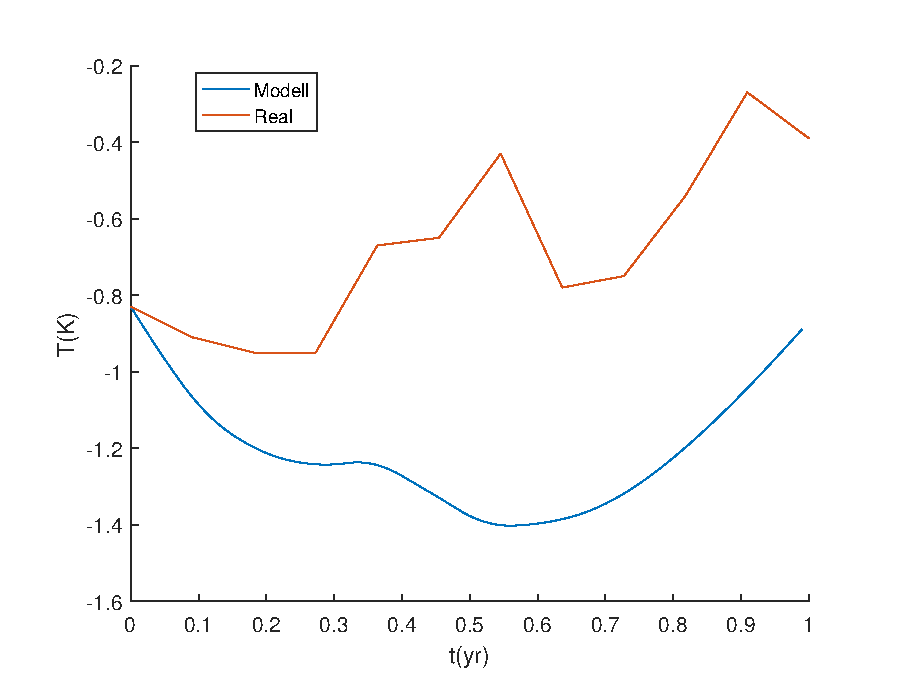
\includegraphics[width=0.66\textwidth,height=0.33\textheight]{verzoegert/inp/figures/sim_1.eps}
	\caption{El-Niño Simulation von 1995-1996 und Vergleich mit realen Daten}
	\label{fig:sim1}
\end{figure}
\begin{figure}
	\centering
	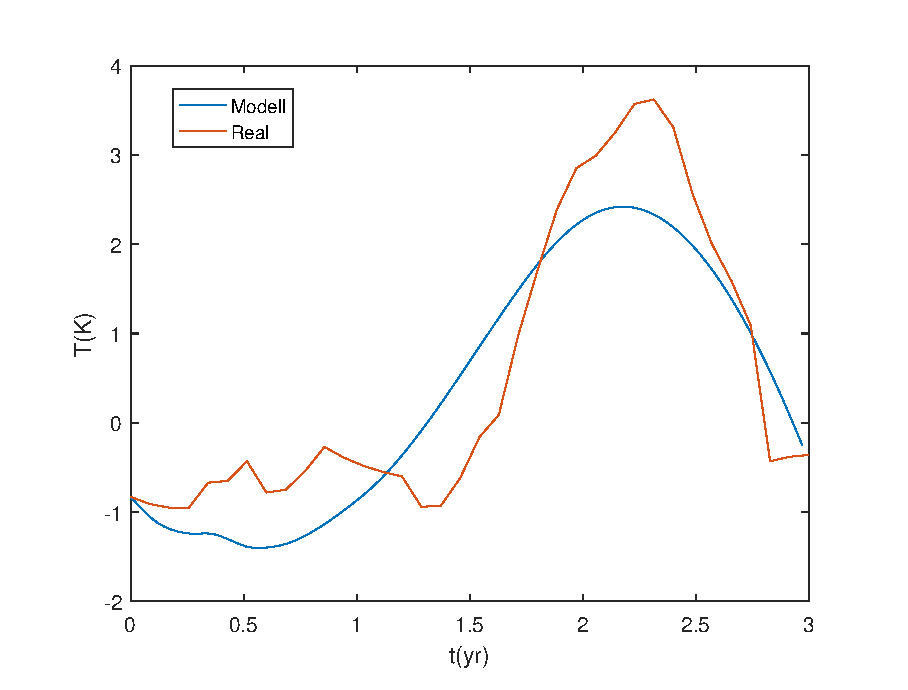
\includegraphics[width=0.66\textwidth,height=0.33\textheight]{verzoegert/inp/figures/sim_3.eps}
	\caption{El-Niño Simulation von 1995-1998 und Vergleich mit realen Daten}
	\label{fig:sim3}
\end{figure}
\begin{figure}
	\centering
	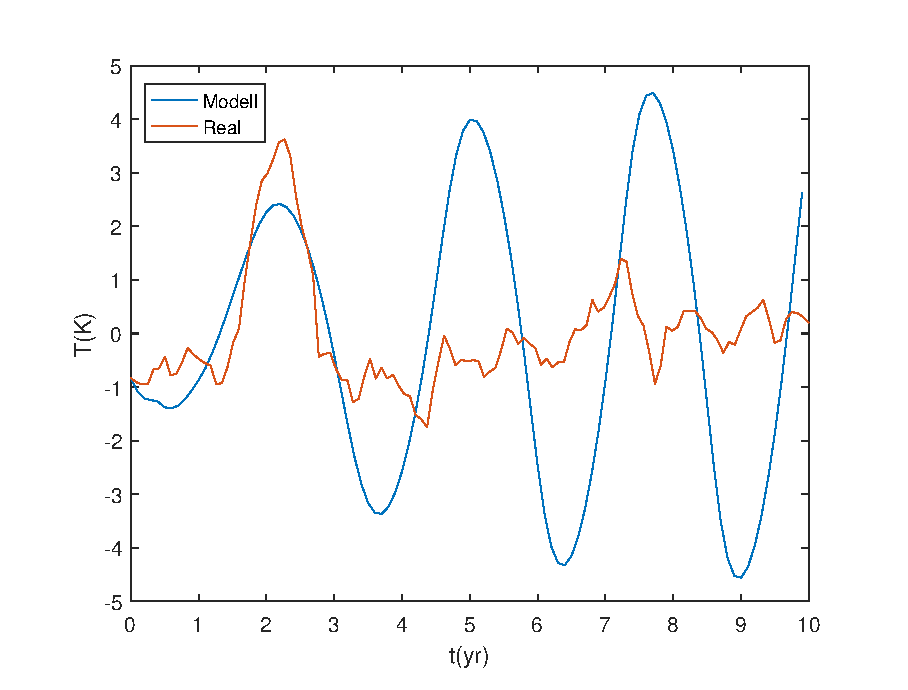
\includegraphics[width=0.66\textwidth,height=0.33\textheight]{verzoegert/inp/figures/sim_10.eps}
	\caption{El-Niño Simulation von 1995-2005 und Vergleich mit realen Daten}
	\label{fig:sim10}
\end{figure}
Mit den richtigen Konstanten lassen sich für kurze Zeiten relativ gute Vorhersagen machen.
Allerdings ist das El-Niño-Phänomen (vgl. Abbildung \ref{fig:elnino}) extrem unkonstant und bräuchte ein komplexeres Modell.
Über längere Zeit versagt das Modell, da es immer zu einer gleichmäßigen Oszillation kommt.

Interessant ist, dass die DDE das kurzfristige Verhalten (1 Jahr, Abbildung \ref{fig:sim1}) richtig berechnet.
Das sieht man an der kurzen Richtungsänderung zwischen 0.3 und 0.4 Jahren.



\subsection{Fazit}
Mit verzögerten Differentialgleichungen können diverse Probleme gelöst werden.
DDEs können analytisch untersucht werden, die Komplexität nimmt allerdings schnell zu.
Eine numerische Simulation ist daher zwingend.
Eine solche Simulation kann relativ einfach erstellt werden und liefert gute Resultate.
Man sollte die Resultate trotzdem genau prüfen, da die Lösungen schnell instabil werden können (vgl. \ref{num:instabil}).

Das Modell zur Modellierung des El-Niño-Phänomens ist sicher noch nicht vollständig.
Es ist aber ein schönes Beispiel einer Anwendung von verzögerten Differentialgleichungen. 

\printbibliography[heading=subbibliography]
\end{refsection}
